%% ==============================
\chapter{\iflanguage{ngerman}{Einleitung}{Introduction}}
\label{sec:Introduction}
%% ==============================



Computergestützte Verfahren werden in der Medizin immer wichtiger. Sie erleichtern dem Arzt seine Arbeit und senken die Wahrscheinlichkeit, dass bei einer Operation ein Fehler gemacht wird.
\newline
Ein Routineprozedur der Neurochirurgie ist die Punktion des Ventrikelsystems zur Drainage von Liquor. Diese wird häufig nötig, wenn ein Patient beispielsweise unter einer Gehirnblutung, einem Schädelhirntrauma oder einem Schlaganfall leidet. Um die Punktion durchzuführen, muss der Chirurg eine Bohrlochtrepanation am sogenannten Kocherpunkt durchführen. Der Arzt muss anhand äußerer anatomischer Landmarker diesen Punkt auf wenige Zentimeter genau finden und die Stichrichtung der Punktion ausmachen. Dieses Verfahren ist sehr fehleranfällig. So kommt es nur in zwei drittel aller Operationen zu einem optimalen Ergebnis, wofür oftmals mehrfach punktiert werden muss. In \autoref{fig:punktion} ist ein Bild eines solche Eingriffs zu sehen. Es ist klar zu erkennen wir der Chirurg mit dem linken Zeigefinger den inneren Augenwinkel zur Orientierung abtastet.


\begin{figure}[!h] 
\centering 
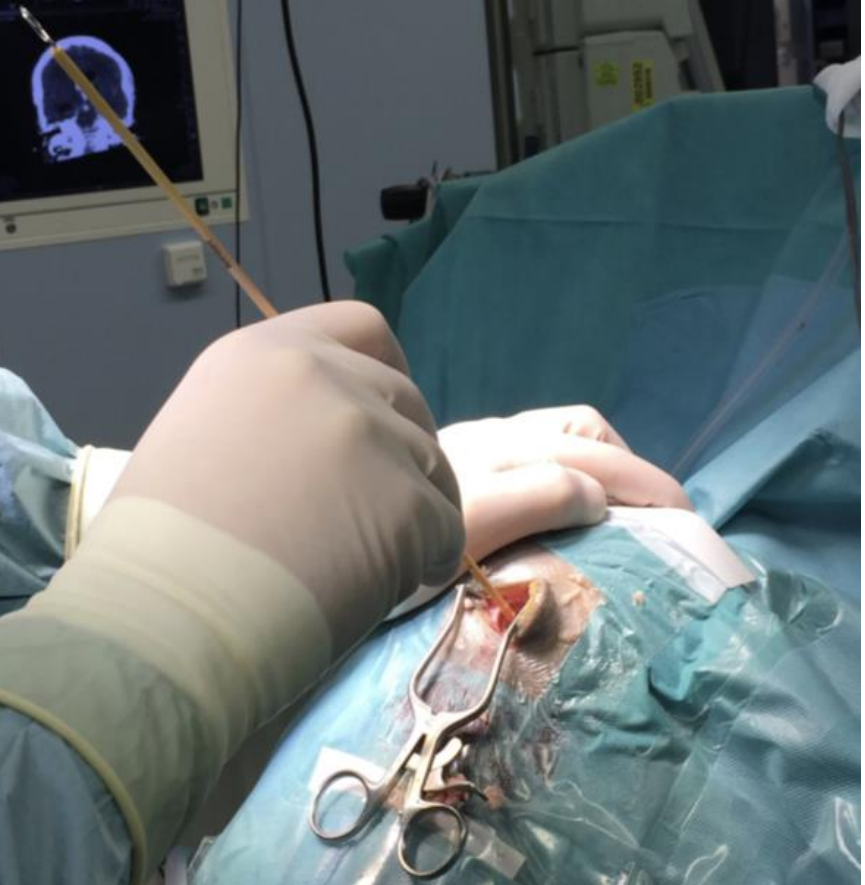
\includegraphics[width=0.6\textwidth]{Logos/Punktion2.png}
\caption{Fotografie einer Ventrikelpunktion  \\Quelle: ...} 
\label{fig:punktion} 
\end{figure}


Im Rahmen des HoloMed Projektes wird daran gearbeitet den Chirurg bei diesem Eingriff zu unterstützen. Der Plan ist es, dass der Arzt mithilfe einer AR-Brille angezeigt bekommt wo sich das Ventrikelsystem befindet und somit mit einer niedrigeren Fehlerwahrscheinlichkeit die Operation durchführen kann.
\newline
Dazu muss zunächst ein CT-Scan des Kopfes gemacht werden. Dieser misst die Absorptionswerte aus verschiedenen Winkeln und erstellt daraus Volumendaten. Diese Absorptionswerte liegen in mehreren Schnittbildern vor.
\newline
Anhand der CT-Daten des Gehirns wird versucht das Ventrikelsystem hervorzuheben und zu visualisieren. Um diese Aufgabe zu lösen eignet sich eine Übergangsfunktion, auch Transferfunktion genannt.
\newline
Allgemein gesprochen ordnet eine Transferfunktion volumetrischen Daten optische Eigenschaften zu. Diese Aufgabe teilt sich in zwei Bereiche auf. Zum einen entscheidet die Funktion welche Daten gezeigt werden und zum anderen wie diese dargestellt werden, beispielsweise welche Farb- und Okklusionswerte diese erhalten. Dabei ist der erste Teil der wesentlich wichtigere und die Farbwahl kann als sekundär betrachtet werden.
\newline
Das Ziel dieser Bachelorarbeit ist es, mithilfe einer geeigneten Transferfunktion das Ventrikelsystem in CT-Daten des Kopfes hervorzuheben.
\newline
Dabei teilt sich der Rest dieser Arbeit folgendermaßen auf. In Kapitel 2, \nameref{sec:state_of_the_art}, wird ein Überblick zu dem aktuellen Stand der Wissenschaft und Technik gegeben, während sich Kapitel 3, \nameref{sec:methods}, mit der in dieser Arbeit verwendeten Methode beschäftigt. In Kapitel 4, \nameref{sec:concept}, wird das Softwaredesign der Implementierung erklärt und in Kapitel 5, \nameref{sec:implementation}, die Implementierung besprochen. Kapitel 6, \nameref{sec:results}, zeigt die Ergebnisse des Verfahrens und evaluiert diese. In Kapitel 7, \nameref{sec:discussion}, wird ein Fazit gezogen und in Kapitel 8, \nameref{sec:conclusion}, werden mögliche Verbesserungen aufgezeigt.